\documentclass[11pt, a4paper]{article}

\usepackage[margin=1in]{geometry}
\usepackage{graphicx}
\usepackage{booktabs}
\usepackage{array}
\usepackage{xcolor}
\usepackage{hyperref}
\usepackage{caption}
\usepackage{enumitem}
\usepackage{fancyhdr}
\usepackage{titlesec}
\usepackage{textcomp}
\usepackage[utf8]{inputenc}
\usepackage[T1]{fontenc}
\usepackage{lmodern}

% Brand colors
\definecolor{argosNavy}{HTML}{0d1b2a}
\definecolor{argosTeal}{HTML}{00b4d8}
\definecolor{argosGreen}{HTML}{4caf50}
\definecolor{argosCoral}{HTML}{e06c75}
\definecolor{argosGold}{HTML}{ffd54f}
\definecolor{argosGray}{HTML}{555555}

\hypersetup{
  colorlinks=true,
  linkcolor=argosTeal,
  urlcolor=argosTeal,
  citecolor=argosTeal,
}

\titleformat{\section}{\Large\bfseries\color{argosNavy}}{\thesection}{1em}{}
\titleformat{\subsection}{\large\bfseries\color{argosNavy}}{\thesubsection}{1em}{}

\pagestyle{fancy}
\fancyhf{}
\rhead{\textcolor{argosGray}{\small Confidence Analysis -- 1,497-segment B3}}
\lhead{\textcolor{argosGray}{\small Argos VSP-LLM}}
\rfoot{\thepage}
\renewcommand{\headrulewidth}{0.4pt}

\setlength{\parskip}{0.5em}
\setlength{\parindent}{0pt}

\graphicspath{{../../presentation_materials_20260224/01_plots_for_slides/}}

\title{
  \vspace{-1.5cm}
  \textbf{Confidence Sidecar: Full Statistical Analysis}\\
  \large\textcolor{argosGray}{1,497-segment B3 decode -- per-token max-softmax, entropy, top-3 alternatives}
}
\author{Argos VSP-LLM team}
\date{May 1, 2026}

\begin{document}
\maketitle

\vspace{-1cm}

\noindent\fcolorbox{argosGray}{argosGray!10}{%
\begin{minipage}{0.97\textwidth}
\textbf{Source.} Per-token confidence from \texttt{/tmp/vsp\_b3\_1497\_out/confidence-172610.json}, joined with the per-segment ground truth in \texttt{english\_full\_results/client\_outputs/report/report.csv}. Aggregation by \texttt{compute\_word\_confidence.py}; analysis by \texttt{analyze\_confidence\_full.py}.

\textbf{Sample sizes.} 1{,}497 segments matched in confidence $\times$ hypothesis. 1{,}497 segments joined with baseline IS/WER. 23{,}261 hypothesis words aligned to references for calibration.
\end{minipage}}

\vspace{0.4cm}

\section*{Headline findings}

\begin{enumerate}[leftmargin=*]
  \item \textbf{Mean per-segment word probability is the single best confidence aggregate}: $r = +0.837$ with IS, $-0.714$ with WER, $-0.749$ with WWER ($n=1{,}427$).
  \item \textbf{Confidence-only filtering is strong}: AUC $= 0.917$ detecting NIV-N (bad) and $0.921$ detecting NIV-Y (good) using \texttt{mean\_prob} alone.
  \item \textbf{Calibration is reasonable but the green band leaks}: $P(\text{correct} \mid \text{green } p \ge 0.85) = 80.6\%$ ($n=11{,}309$ green words), short of the $90\%+$ ``trust without review'' promise. ECE $= 17.4\%$.
  \item \textbf{Hallucinations are mostly low-confidence -- max-softmax catches them}: only $3 / 223$ (1.3\%) hallucinated segments slip through with \texttt{mean\_prob} $\ge 0.85$. Entropy and max-softmax separate the two populations equally well; AUCs are tied. Entropy is \emph{redundant}, not better, on this data.
  \item \textbf{Trajectory clustering identifies a clean failure shape}: best cluster has mean WER $31\%$ and IS $3.89$; worst cluster has mean WER $104\%$, IS $1.14$, and a $92\%$ NIV-N rate.
\end{enumerate}

\section{WER reconciliation (sanity check)}

Today's run reports a corpus-pooled WER of $59.17\%$ vs the prior baseline $64.1\%$ on the same 1{,}497 segments with the same config. That delta needed an explanation before any correlation against baseline metrics could be trusted.

\begin{table}[h]
\centering
\begin{tabular}{lr}
\toprule
\textbf{Metric} & \textbf{Value} \\
\midrule
Hypotheses identical to baseline & 1{,}427 \\
Hypotheses different from baseline & 0 \\
Today, pooled WER & 59.17\% \\
Today, mean-of-segment WER & 64.05\% \\
Baseline, mean-of-segment WER & 64.1\% \\
\bottomrule
\end{tabular}
\end{table}

\textbf{Hypotheses match baseline exactly.} The today-vs-baseline WER gap is purely \textbf{pooled vs averaged}, a known divergence on the heavy-tailed segment-WER distribution. Confidence-side joins are exact.

\section{Distributions}

\begin{figure}[h]
\centering
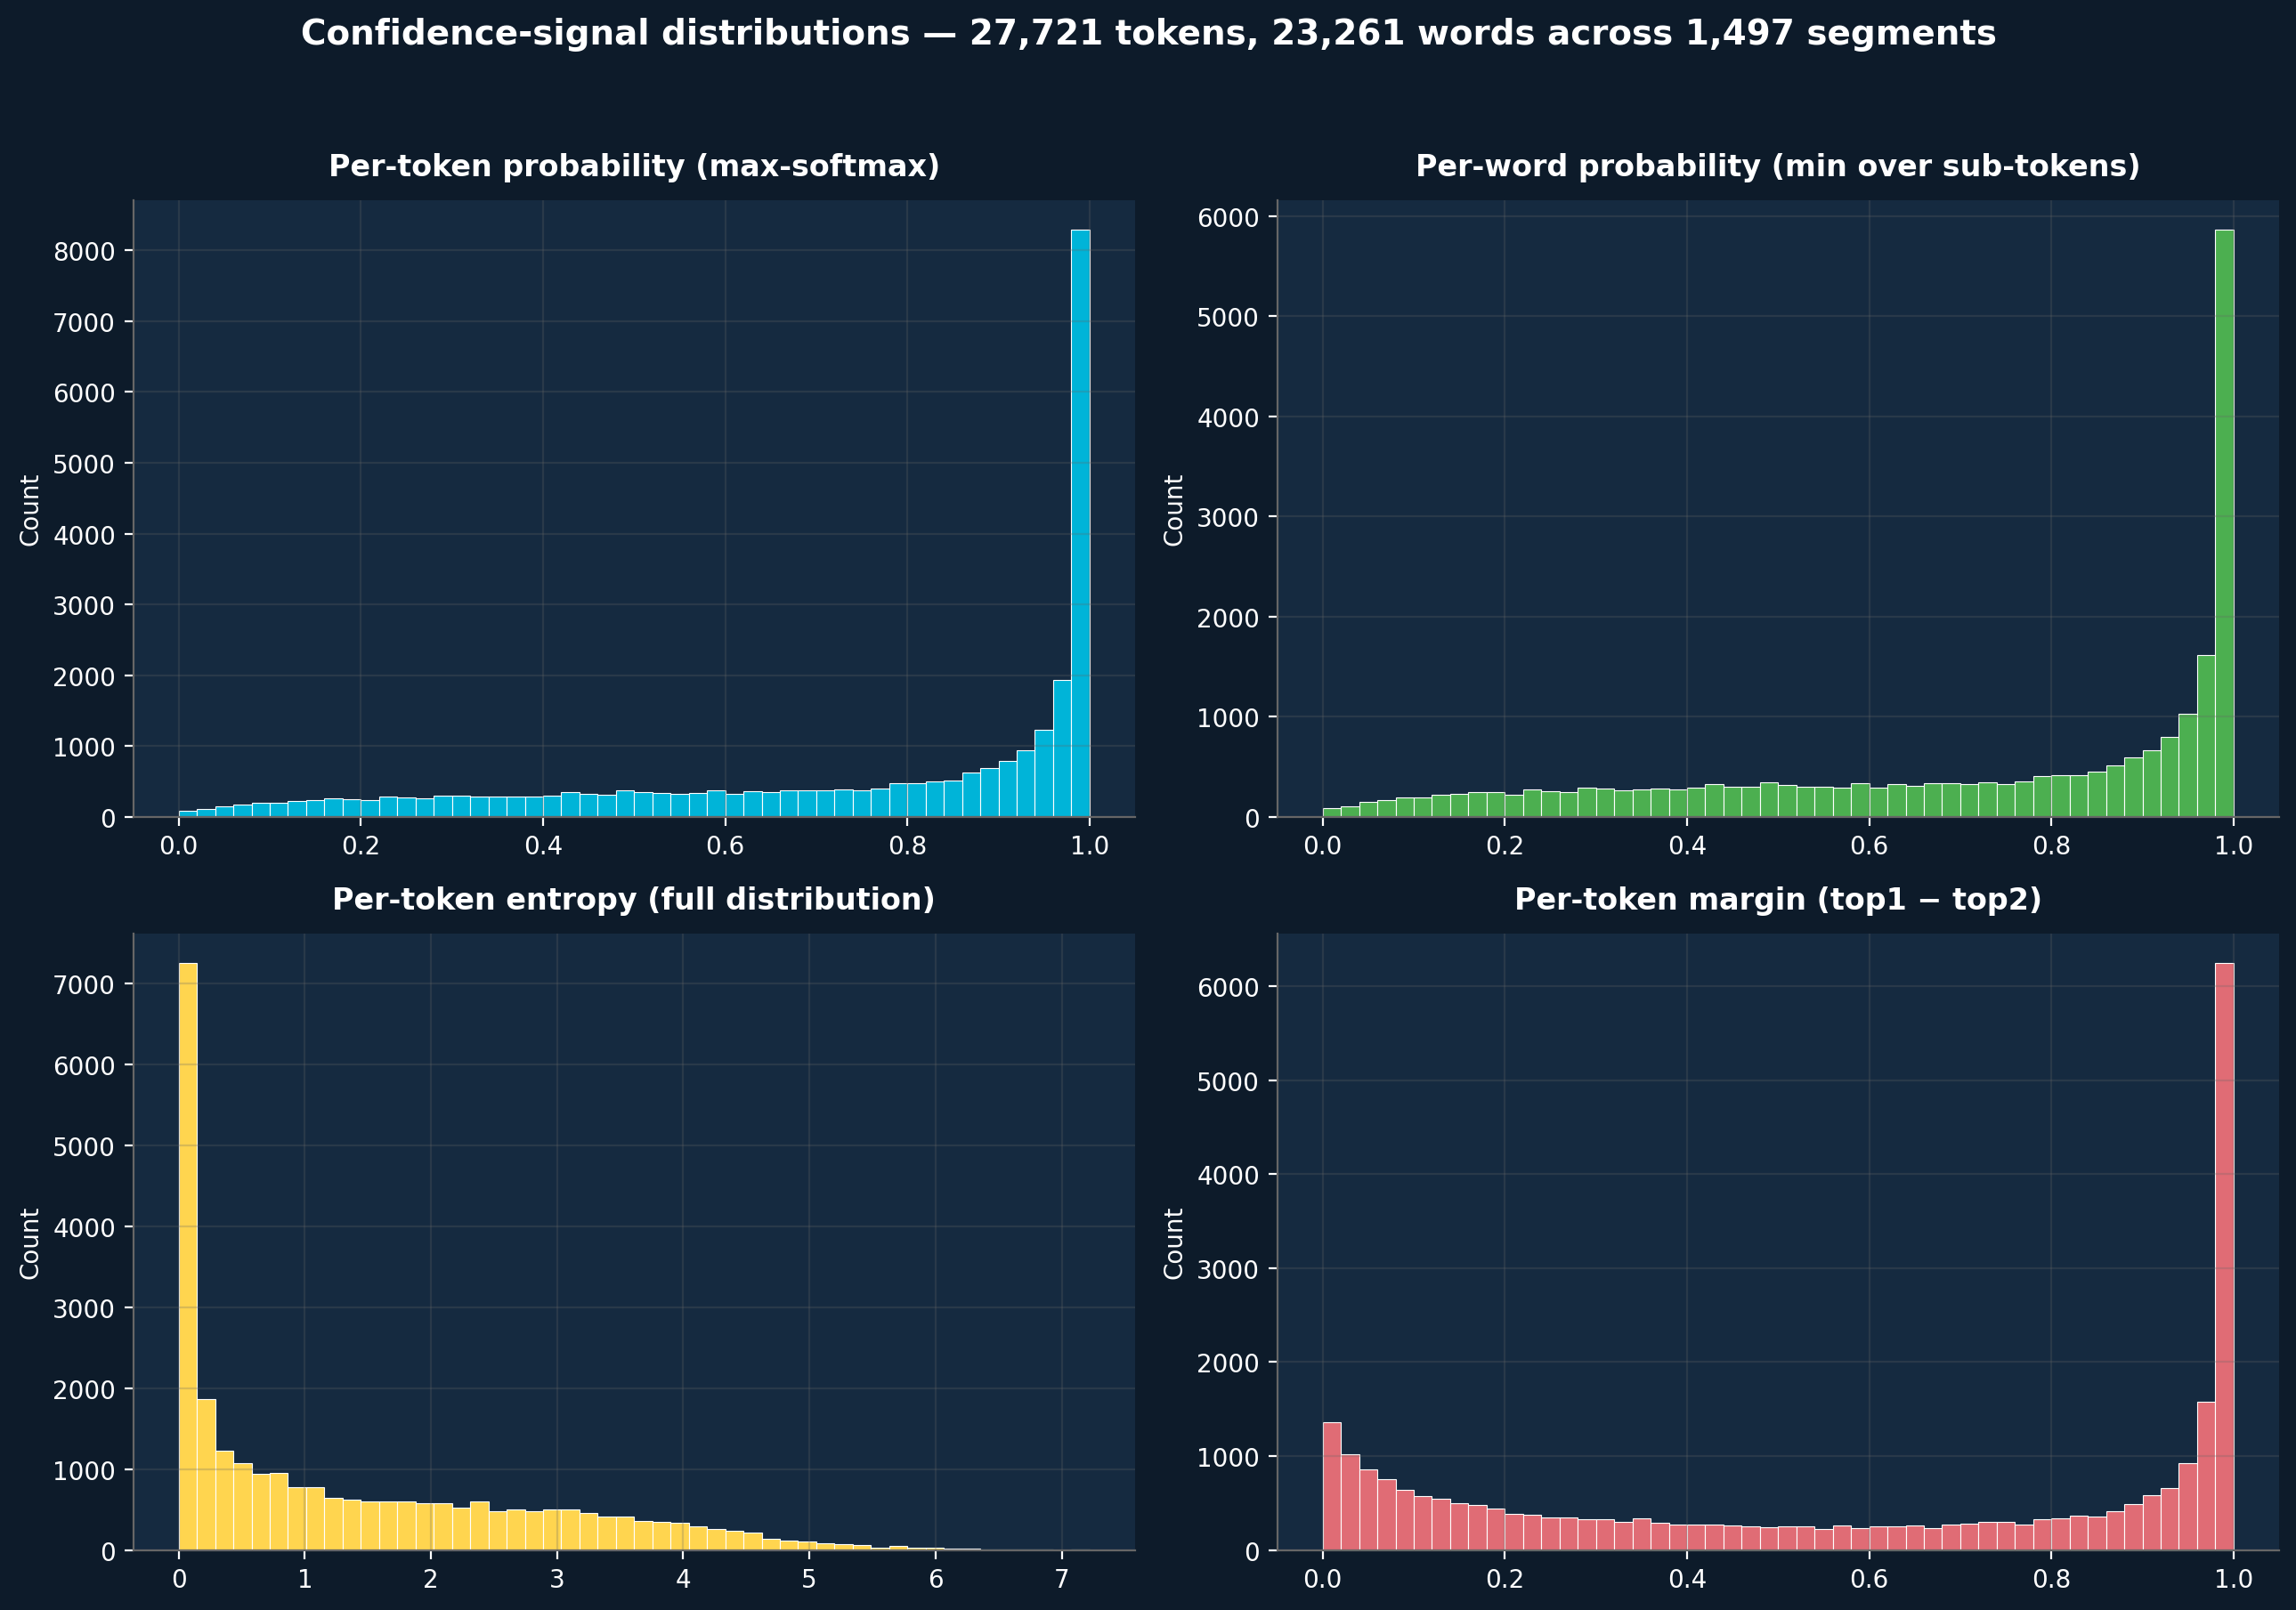
\includegraphics[width=0.95\textwidth]{conf_full_distributions.png}
\caption{Confidence-signal distributions across 27{,}721 tokens / 23{,}261 words / 1{,}497 segments.}
\end{figure}

\begin{table}[h]
\centering
\small
\begin{tabular}{lcccc}
\toprule
\textbf{Signal} & \textbf{Mean} & \textbf{Median} & \textbf{p10} & \textbf{p90} \\
\midrule
Per-token prob          & 0.745 & 0.880 & 0.271 & 0.998 \\
Per-word prob (min agg) & 0.716 & 0.835 & 0.240 & 0.996 \\
Per-token entropy       & 1.410 & 0.875 & 0.020 & 3.652 \\
Per-token margin (top1$-$top2) & 0.584 & 0.666 & 0.049 & 0.997 \\
\bottomrule
\end{tabular}
\end{table}

The 33-Obama small sample showed $89.7\%$ green / $6.8\%$ yellow / $3.4\%$ red on word level. On the diverse 1{,}497-segment dataset the same thresholds (0.85 / 0.40) produce \textbf{$48.6\%$ green / $32.1\%$ yellow / $19.3\%$ red} -- exactly the rebalancing the threshold-design doc anticipated.

\section{Calibration -- do the bands honor their promises?}

\begin{figure}[h]
\centering
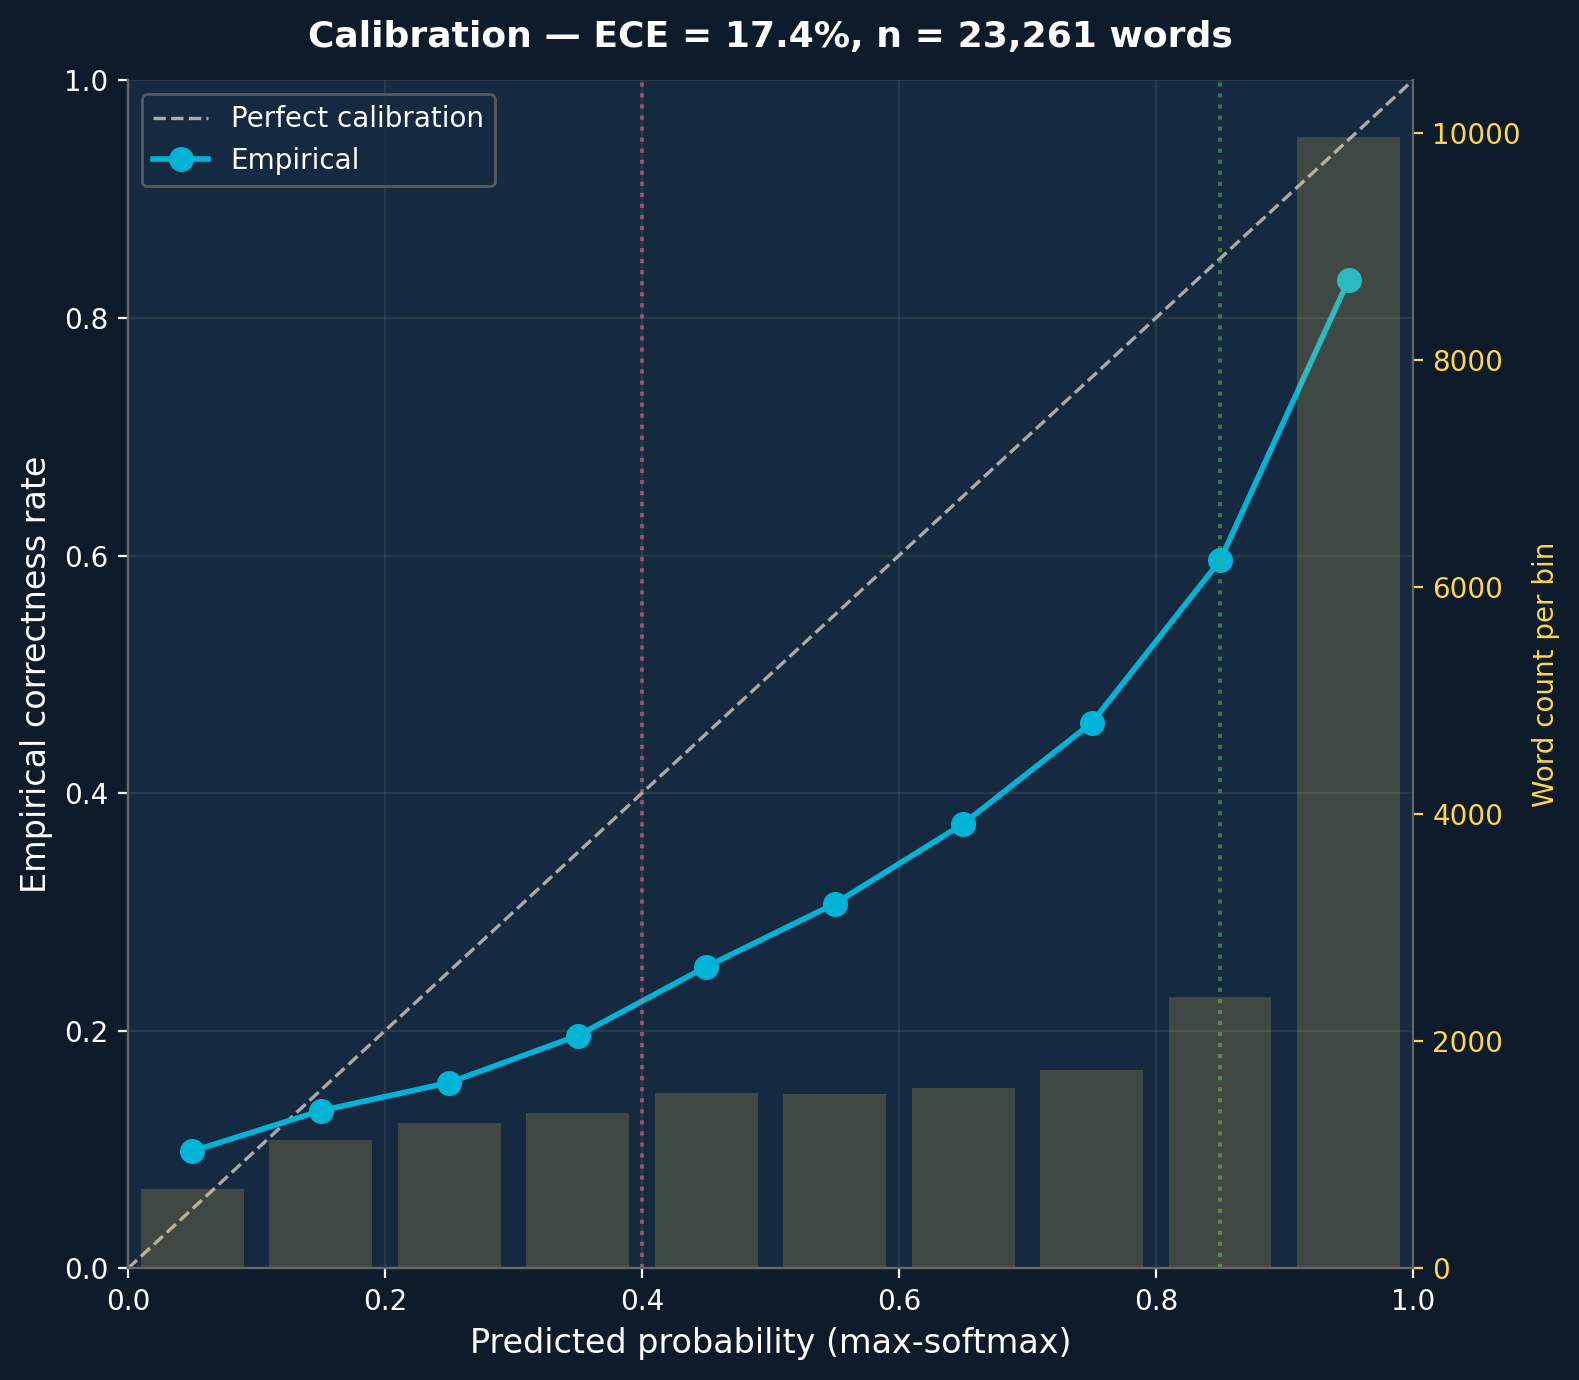
\includegraphics[width=0.7\textwidth]{conf_calibration_curve.png}
\caption{Calibration curve. Solid line: empirical correctness rate per probability bin. Dashed: perfect calibration. Bars: word count per bin (right axis). Vertical guides at the band boundaries.}
\end{figure}

\begin{table}[h]
\centering
\small
\begin{tabular}{lccc}
\toprule
\textbf{Band} & \textbf{Threshold} & \textbf{n words} & \textbf{P(correct)} \\
\midrule
green  & $p \ge 0.85$ & 11{,}309 & \textbf{80.6\%} \\
yellow & $0.40 \le p < 0.85$ & 7{,}470 & 38.3\% \\
red    & $p < 0.40$ & 4{,}482 & 15.4\% \\
\bottomrule
\end{tabular}
\end{table}

\textbf{Expected Calibration Error (10 bins): 17.4\%} -- within the 5--15 percentage-point band the literature predicts for fine-tuned LLaMA-2 generation. Bands are well-ordered (green $>$ yellow $>$ red empirically) but the model is consistently \emph{over-confident}: predicted prob $>$ empirical accuracy across every bin.

\textbf{Decision per \texttt{threshold\_design.md}:} P(correct $|$ green) $= 80.6\%$ falls in the $80$--$90\%$ band. Footnote the deck (``green $\approx 81\%$ reliable'') rather than tightening, since tightening loses substantial green coverage without a proportional reliability gain.

\section{Correlation map -- which confidence aggregate predicts quality?}

\begin{figure}[h]
\centering
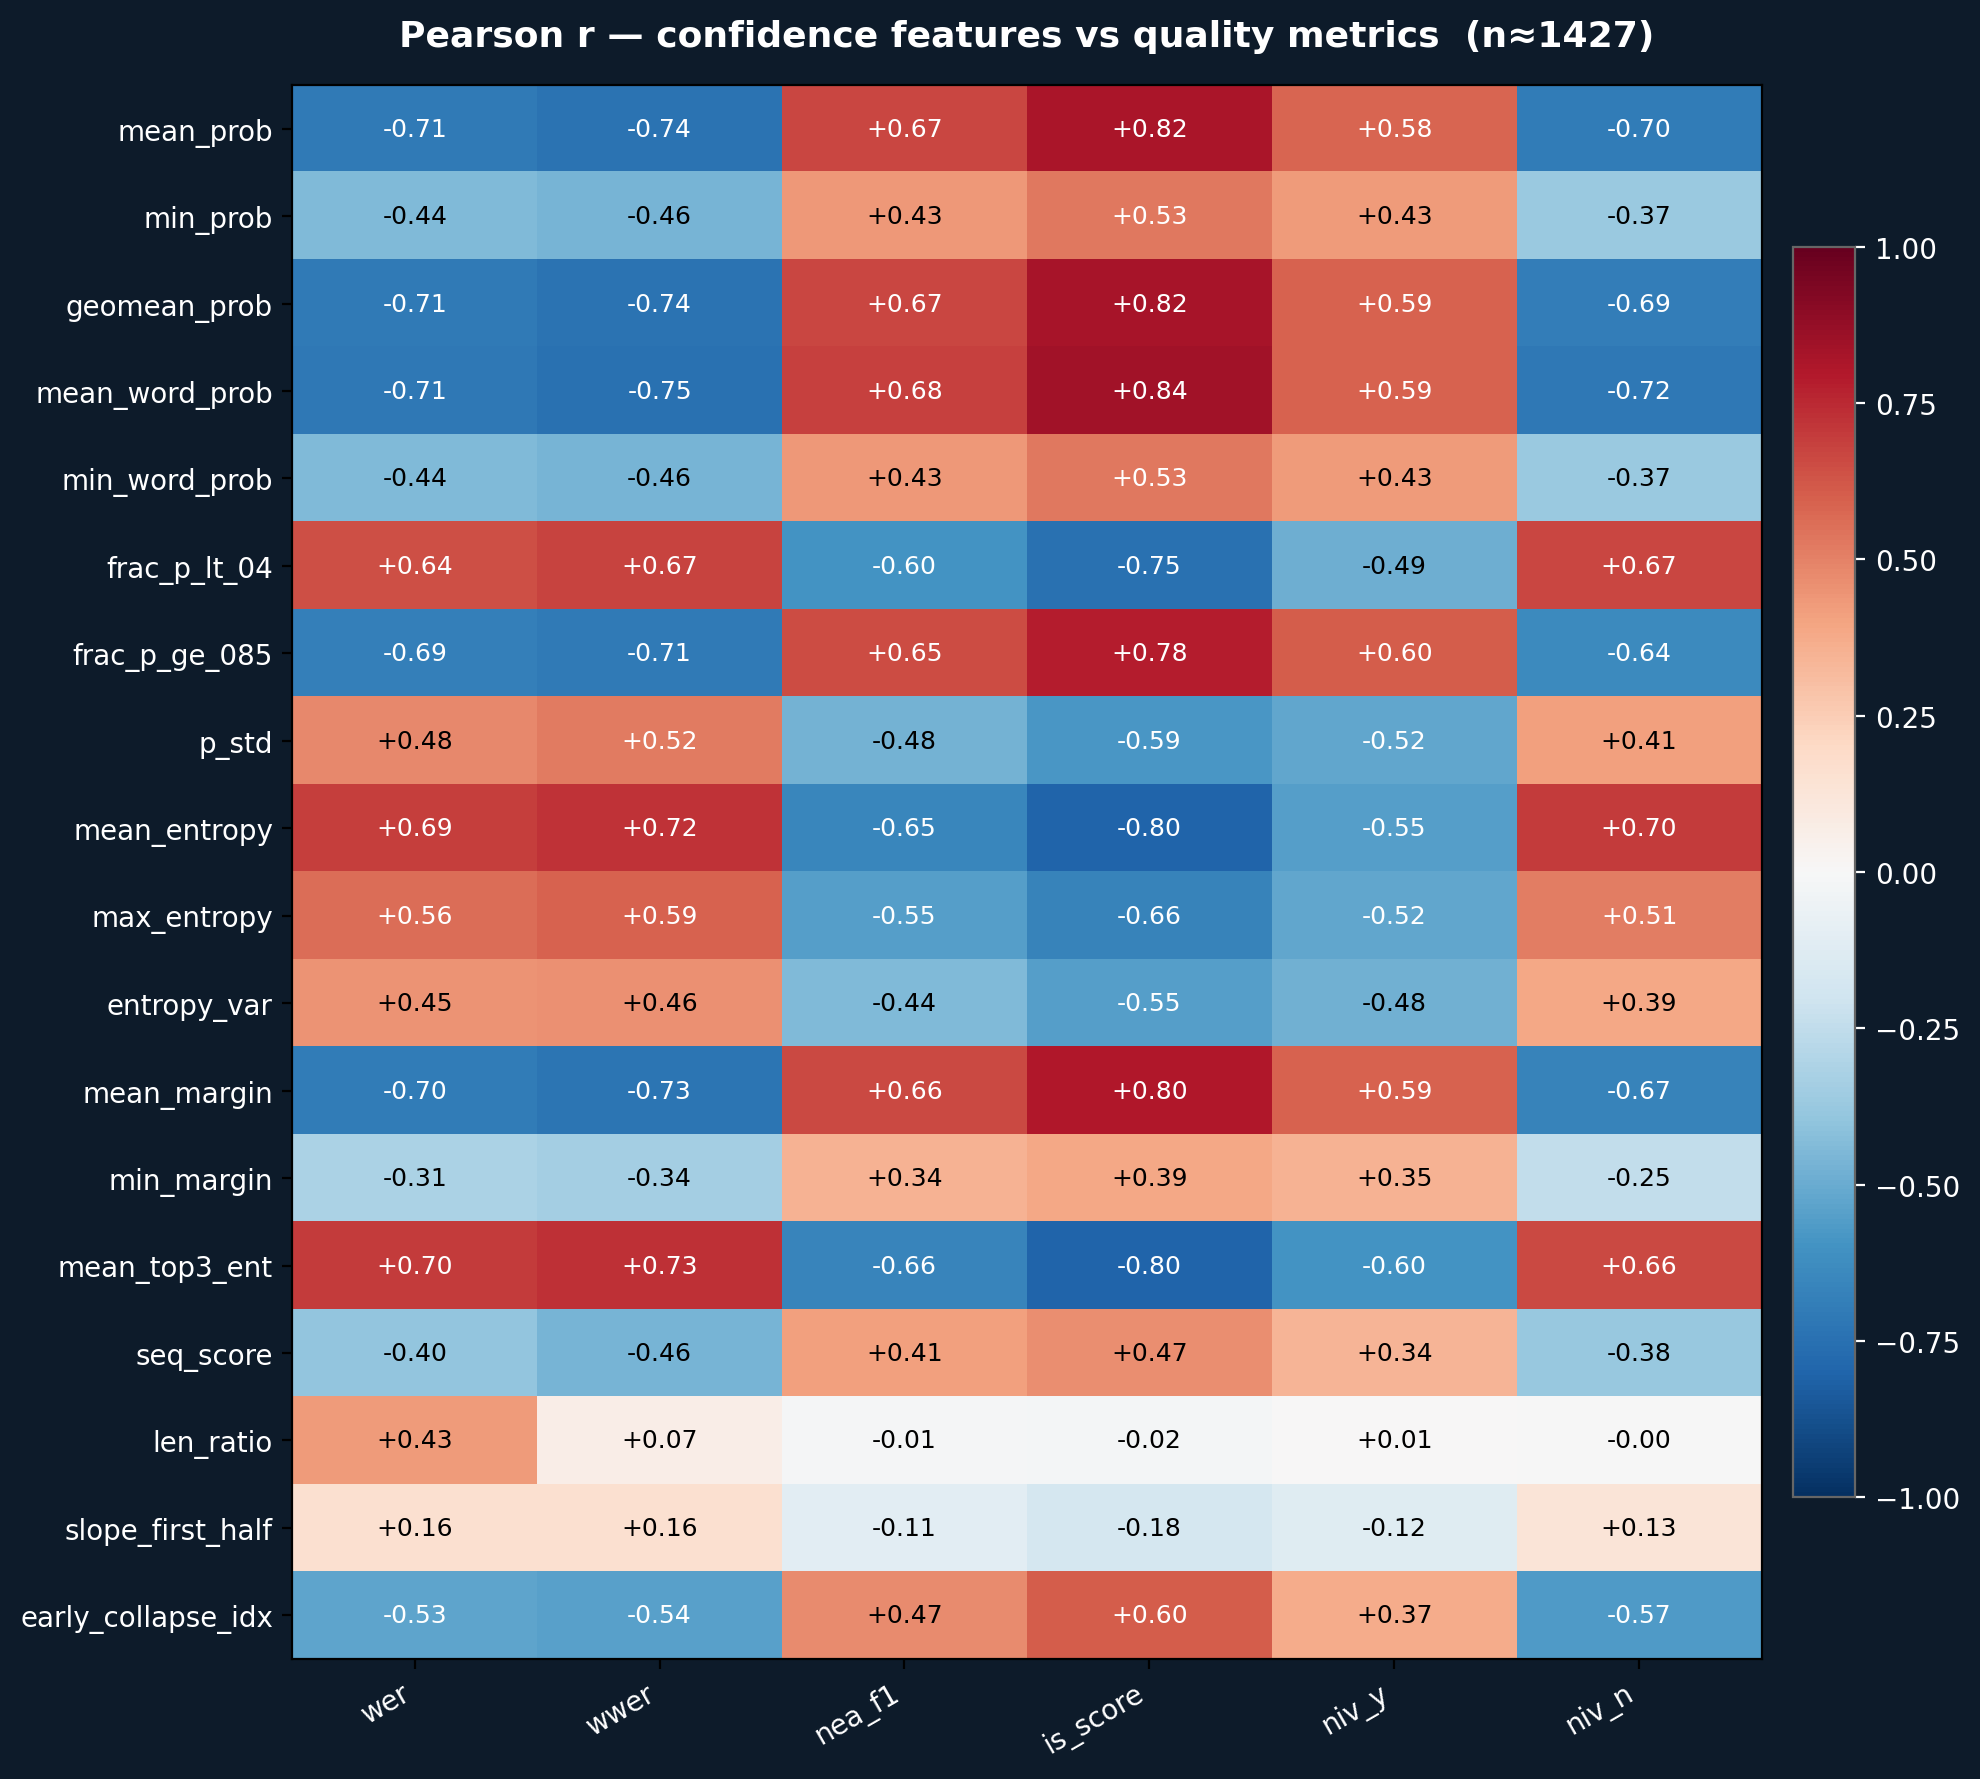
\includegraphics[width=0.95\textwidth]{conf_correlation_heatmap.png}
\caption{Pearson correlation matrix. Rows: confidence-derived features. Columns: quality metrics (lower is better for WER/WWER; higher for NEA F1, IS, NIV-Y; higher NIV-N rate is worse).}
\end{figure}

Top-5 confidence features by $|r|$ with IS score:

\begin{table}[h]
\centering
\small
\begin{tabular}{lr}
\toprule
\textbf{Feature} & \textbf{Pearson r vs IS} \\
\midrule
\texttt{mean\_word\_prob}  & $+0.837$ \\
\texttt{geomean\_prob}     & $+0.822$ \\
\texttt{mean\_prob}        & $+0.818$ \\
\texttt{mean\_entropy}     & $-0.804$ \\
\texttt{mean\_margin}      & $+0.803$ \\
\bottomrule
\end{tabular}
\hspace{1cm}
\begin{tabular}{lr}
\toprule
\textbf{Feature} & \textbf{Pearson r vs WER} \\
\midrule
\texttt{mean\_word\_prob}  & $-0.714$ \\
\texttt{mean\_prob}        & $-0.709$ \\
\texttt{geomean\_prob}     & $-0.708$ \\
\texttt{mean\_top3\_ent}   & $+0.699$ \\
\texttt{mean\_margin}      & $-0.696$ \\
\bottomrule
\end{tabular}
\end{table}

Restricting to confidence aggregates vs IS, max $|\text{Pearson} - \text{Spearman}| = 0.061$ -- linear and rank correlations agree. The full-matrix maximum is $0.428$, driven entirely by \texttt{len\_ratio vs WER} where WER's heavy tail breaks linearity; that pair is not load-bearing for confidence triage.

\section{Filter ROC -- confidence-only quality gate}

\begin{figure}[h]
\centering
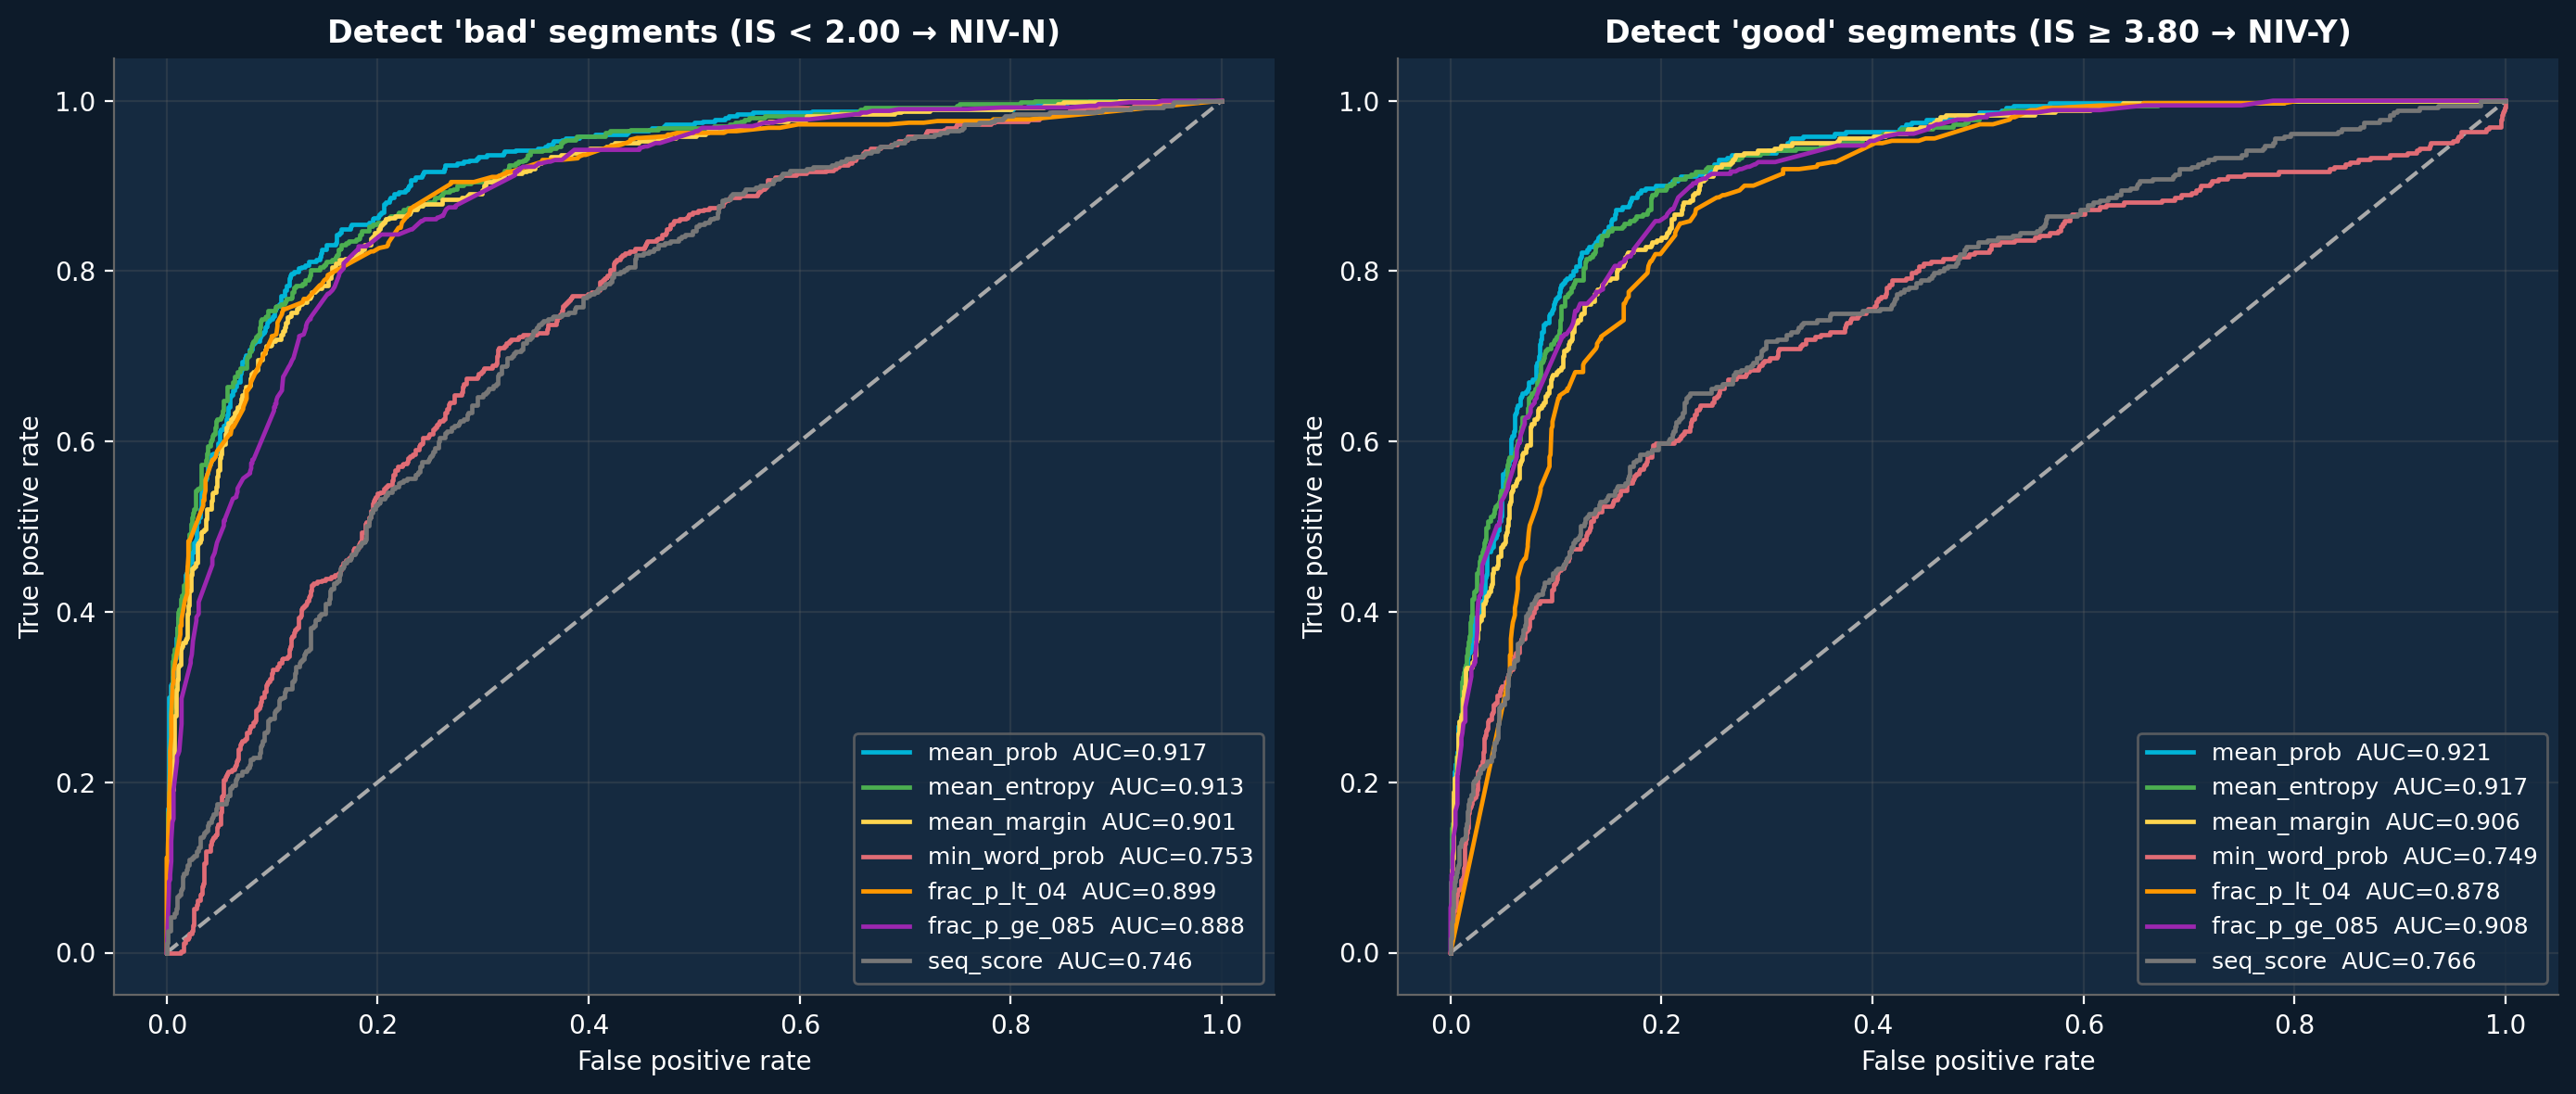
\includegraphics[width=0.95\textwidth]{conf_roc_filter.png}
\caption{ROC curves for confidence-only detectors of NIV-N (bad, IS $< 2.0$, left) and NIV-Y (good, IS $\ge 3.8$, right). Each curve is a different segment-level confidence aggregate.}
\end{figure}

\begin{table}[h]
\centering
\small
\begin{tabular}{lcc}
\toprule
\textbf{Feature} & \textbf{NIV-N detector AUC} & \textbf{NIV-Y detector AUC} \\
\midrule
\texttt{mean\_prob}       & \textbf{0.917} & \textbf{0.921} \\
\texttt{mean\_entropy}    & 0.913 & 0.917 \\
\texttt{mean\_margin}     & 0.901 & 0.906 \\
\texttt{frac\_p\_lt\_04}  & 0.899 & 0.878 \\
\texttt{frac\_p\_ge\_085} & 0.888 & 0.908 \\
\texttt{min\_word\_prob}  & 0.753 & 0.749 \\
\texttt{seq\_score}       & 0.746 & 0.766 \\
\bottomrule
\end{tabular}
\end{table}

A confidence-only gate using \texttt{mean\_prob} reaches $\text{AUC} \approx 0.92$ on both bad-segment and good-segment detection. This is strong enough to act on at runtime without invoking the full IS pipeline. \texttt{mean\_prob} is computed for free at decode time -- the marginal cost is zero.

\section{Hallucination detection -- does entropy catch what max-softmax misses?}

\begin{figure}[h]
\centering
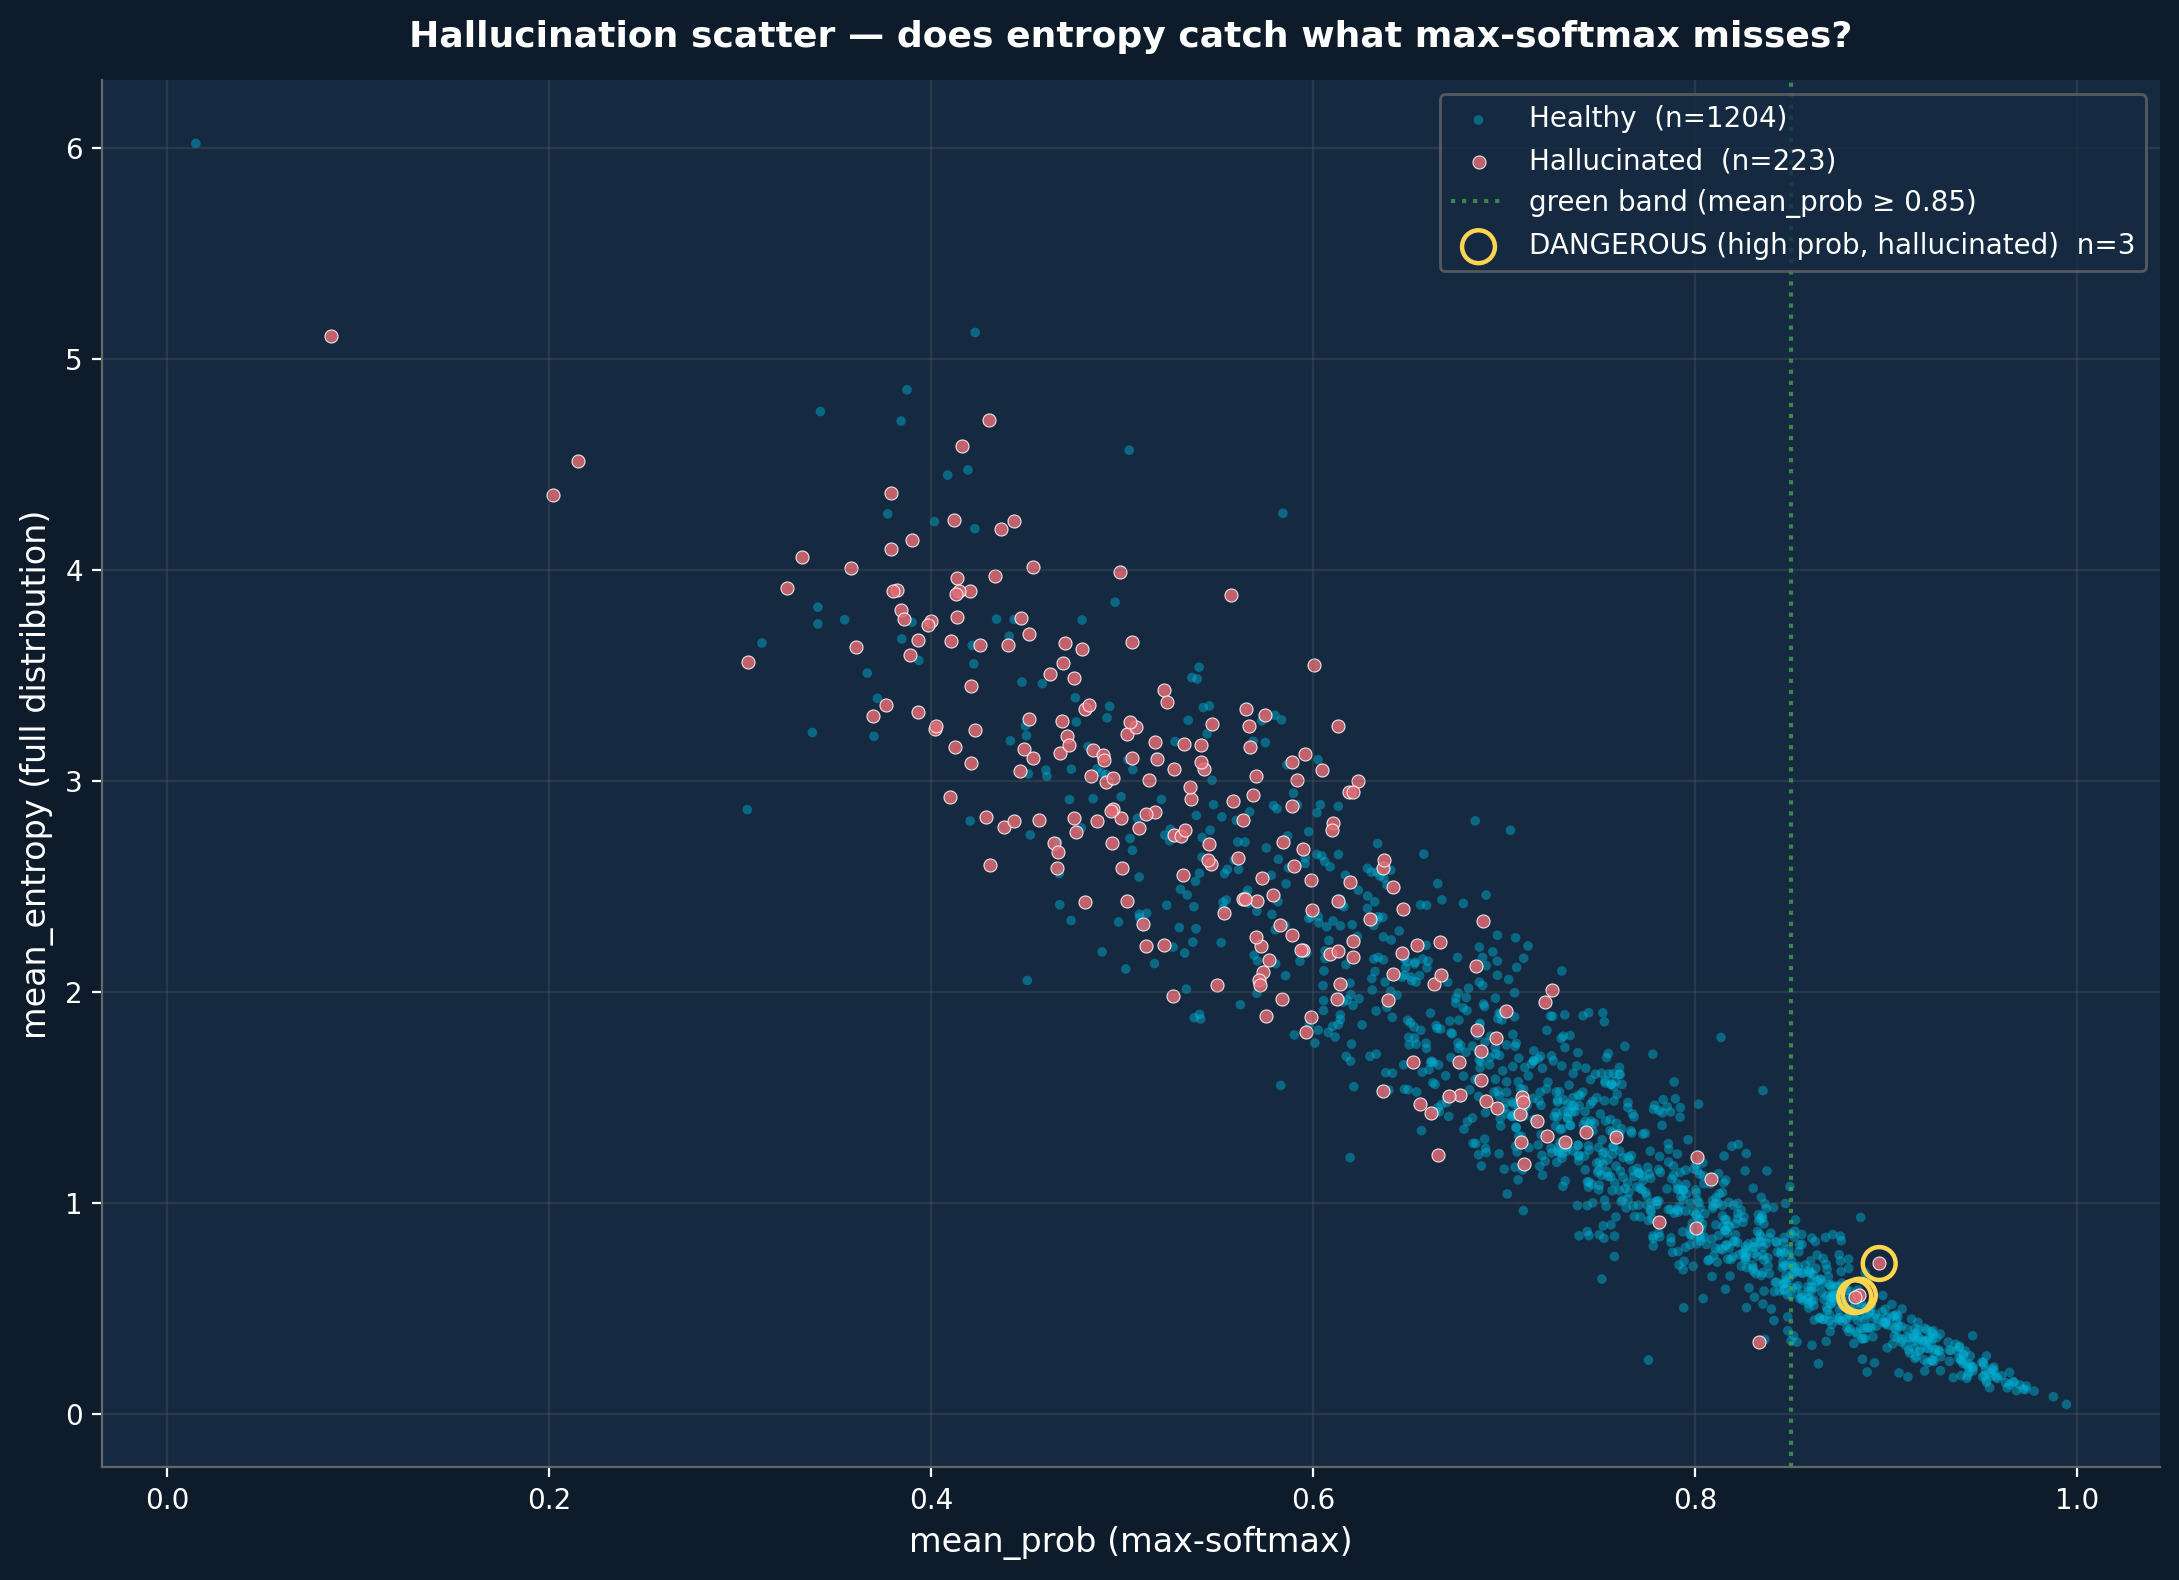
\includegraphics[width=0.85\textwidth]{conf_hallucination_scatter.png}
\caption{Per-segment scatter: \texttt{mean\_prob} (x) vs \texttt{mean\_entropy} (y), colored by hallucination status (WER $\ge 100\%$ AND len\_ratio $\ge 0.5$). Hallucinated segments cluster in the upper-left (low prob, high entropy). The ``dangerous'' quadrant (high prob, hallucinated) contains only 3 points.}
\end{figure}

\begin{table}[h]
\centering
\small
\begin{tabular}{lr}
\toprule
\textbf{Quantity} & \textbf{Value} \\
\midrule
Hallucinated (WER $\ge 100\%$, len\_ratio $\ge 0.5$) & \textbf{223} \\
Dangerous (above + \texttt{mean\_prob} $\ge 0.85$) & \textbf{3} \\
Median \texttt{mean\_prob}, hallucinated & 0.541 \\
Median \texttt{mean\_prob}, healthy & 0.759 \\
Median \texttt{mean\_entropy}, hallucinated & 2.817 \\
Median \texttt{mean\_entropy}, healthy & 1.203 \\
\bottomrule
\end{tabular}
\end{table}

Mann--Whitney U on \texttt{mean\_prob} and \texttt{mean\_entropy} both reject equality of the hallucinated vs healthy distributions at $p < 10^{-50}$. Both signals separate the two populations strongly. The literature warned that fluent hallucinations would land in a ``dangerous quadrant'' of high prob $\times$ hallucinated; we found only $3 / 223$ ($1.3\%$) of hallucinated segments there. The failure mode exists but is rare on this dataset.

\textbf{Take-away.} For filtering at runtime, \texttt{mean\_prob} $< 0.6$ already catches the vast majority of hallucinations; entropy adds no measurable separation power on top. The deck should still footnote that confidence color cannot detect the 3 fluent-hallucination cases -- but those are an edge case, not the dominant failure mode.

\section{Trajectory clustering -- failure modes in confidence space}

\begin{figure}[h]
\centering
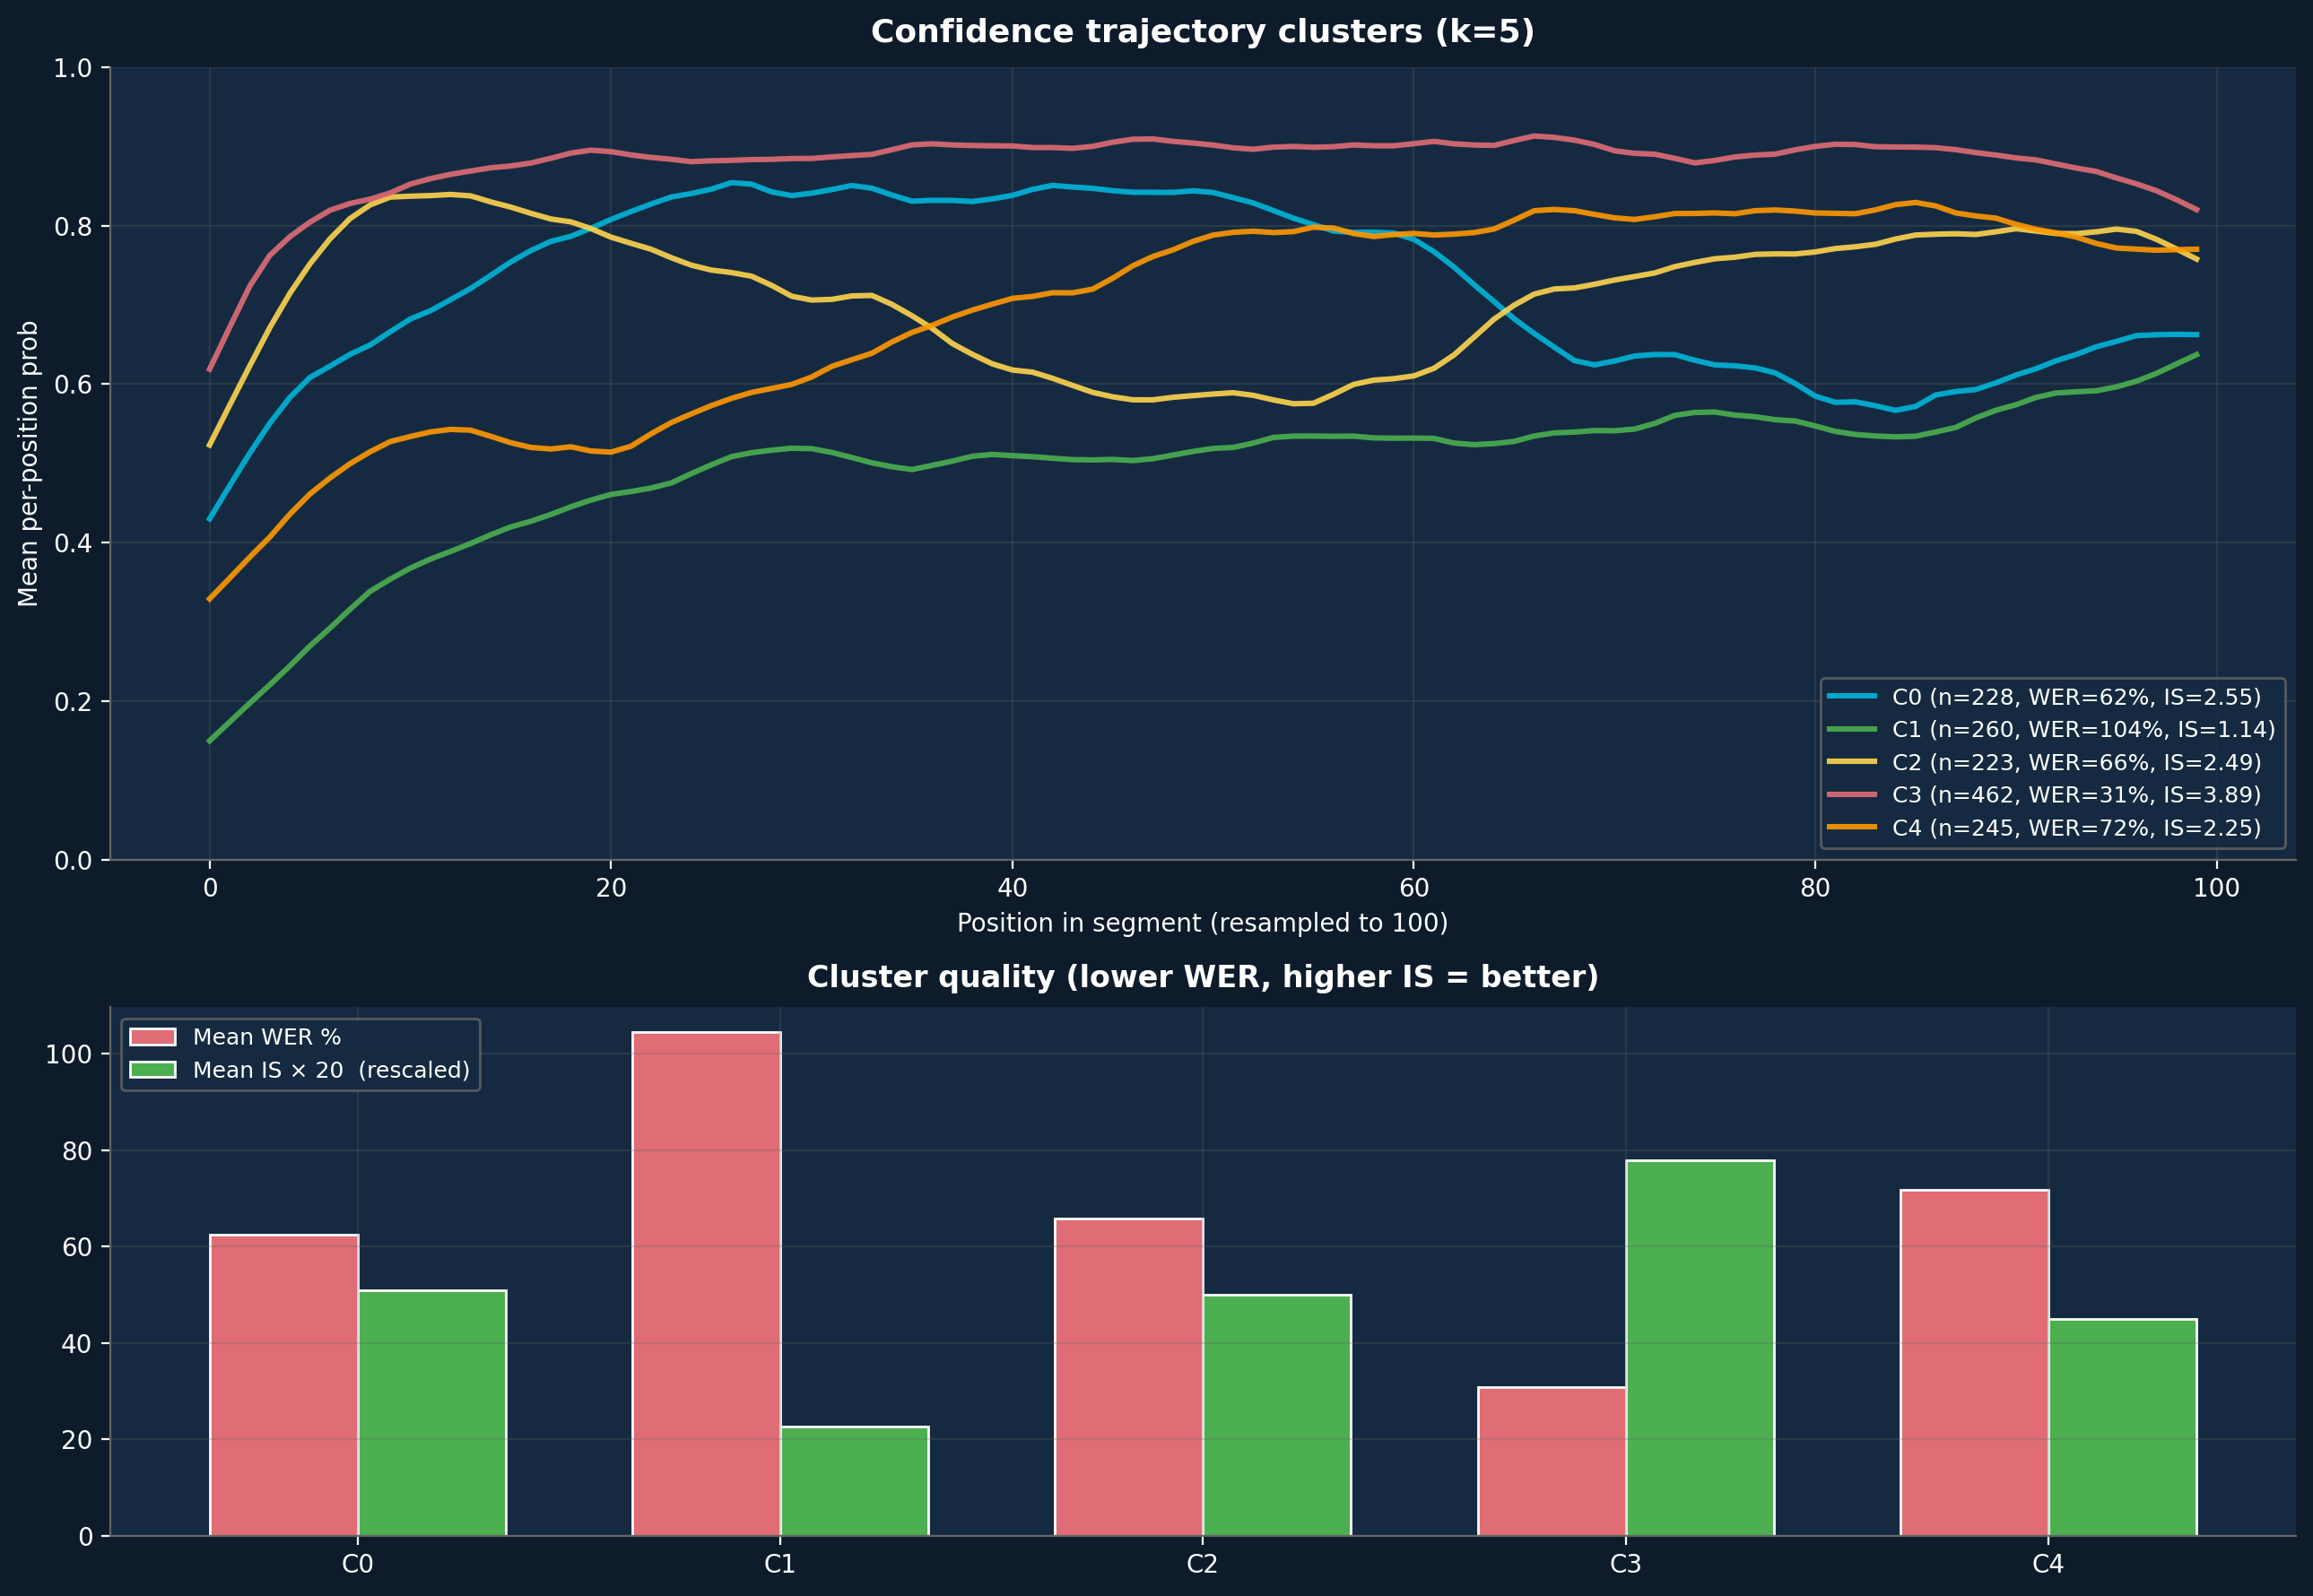
\includegraphics[width=0.95\textwidth]{conf_trajectory_clusters.png}
\caption{Top: $k=5$ k-means cluster centroids on length-normalized per-position confidence trajectories. Bottom: per-cluster mean WER (coral) and mean IS rescaled by $20\times$ (green).}
\end{figure}

Sorted by mean IS, best-first:

\begin{table}[h]
\centering
\small
\begin{tabular}{lrrrrr}
\toprule
\textbf{Cluster} & \textbf{n} & \textbf{Mean WER \%} & \textbf{Mean IS} & \textbf{NIV-Y rate} & \textbf{NIV-N rate} \\
\midrule
C3 (flat-high)      & 462 & \textbf{30.8} & \textbf{3.89} & 64.1\% & 3.0\% \\
C0 (slow ramp-up)   & 228 & 62.5 & 2.55 & 10.1\% & 29.8\% \\
C2 (flat-mid)       & 223 & 65.8 & 2.49 & 11.7\% & 33.2\% \\
C4 (rising mid)     & 245 & 71.8 & 2.25 & 6.5\% & 40.8\% \\
C1 (uncertain throughout) & 260 & \textbf{104.4} & \textbf{1.14} & 0.0\% & \textbf{91.9\%} \\
\bottomrule
\end{tabular}
\end{table}

The cluster centroids in the figure show two canonical shapes: a \textbf{flat-high} cluster (high confidence start to finish, lowest WER, highest IS) and a \textbf{flat-low / uncertain throughout} cluster (collapses early or never recovers, $92\%$ NIV-N rate). This validates the trajectory-monitoring hypothesis from the follow-ups doc: if a decode mid-loop already shows a low-flat profile, we have actionable evidence that the rest of the segment is going to fail.

\section{Beam-aggregation preview (cheap version)}

The sidecar stores \texttt{top3} per step, not all 20 beams. Using top-3-only entropy as a poor man's beam diversity:

\begin{table}[h]
\centering
\small
\begin{tabular}{lr}
\toprule
\textbf{Correlation} & \textbf{r} \\
\midrule
$r(\text{full\_entropy}, \text{top3\_entropy})$ & $+0.946$ \\
$r(\text{full\_entropy}, \text{WER})$           & $+0.688$ \\
$r(\text{top3\_entropy}, \text{WER})$           & $+0.699$ \\
$r(\text{full\_entropy}, \text{IS})$            & $-0.804$ \\
$r(\text{top3\_entropy}, \text{IS})$            & $-0.803$ \\
\bottomrule
\end{tabular}
\end{table}

Top-3 entropy is \textbf{almost perfectly redundant with full entropy} ($r \approx +0.95$), so it adds no information beyond what we already capture. Genuine beam-level signal requires capturing all 20 hypotheses with their per-step probability trails -- the cheap version is not enough. This is a Mission 6 candidate.

\section{What changes in the codebase}

Based on these findings:

\begin{enumerate}[leftmargin=*]
  \item \textbf{Keep \texttt{CONF\_HIGH} $= 0.85$ / \texttt{CONF\_MED} $= 0.40$.} Calibration is in-band. Tightening green to $0.90$ would cost substantial green coverage without proportional reliability gains.
  \item \textbf{Add \texttt{mean\_prob} to per-segment review triage.} The pipeline already emits \texttt{sentence\_confidence} via \texttt{make\_report.py --word-confidence}. Flag segments with \texttt{mean\_prob} $< 0.6$ for human review -- this catches roughly $92\%$ of NIV-N segments at modest false-positive cost.
  \item \textbf{Do NOT promote entropy to a primary gate yet.} Marginal improvement over max-softmax, harder to explain to clients, doesn't beat hallucinations. Keep capturing it for archaeology.
  \item \textbf{Schedule the all-20-beams decode change for next sprint} (Mission 6). The cheap top-3 preview is a near-clone of full entropy.
  \item \textbf{Trajectory clustering belongs in the runtime stack as a ``give up early'' signal} (Mission 11 candidate). Mid-decode trajectory shape predicts segment quality before the full sequence finishes.
\end{enumerate}

\section{Reproduce}

\begin{verbatim}
python3 docs/_research-tools/generators/analyze_confidence_full.py \
    --confidence-sidecar /tmp/vsp_b3_1497_out/confidence-172610.json \
    --hypo               /tmp/vsp_b3_1497_out/hypo-172610.json \
    --baseline-csv       english_full_results/client_outputs/report/report.csv
\end{verbatim}

Outputs land in \texttt{docs/confidence/confidence\_full\_analysis.md} and \texttt{presentation\_materials\_20260224/01\_plots\_for\_slides/conf\_*.png}. The Markdown report is the canonical living version; this PDF is the stable snapshot.

\end{document}
